\documentclass[12pt, svgnames]{article}

\usepackage{xcolor}
\usepackage{colortbl}
\usepackage{amssymb}
\usepackage{fullpage}
\usepackage[round,numbers]{natbib}
\usepackage{multirow}
\usepackage{longtable}
\usepackage{booktabs}
\usepackage{graphicx}
\usepackage{float}
\usepackage{../ltx/edcomms}
%%\usepackage{../ltx/setupComments}
\usepackage{hyperref}
\usepackage{geometry}
\usepackage{changepage}
\usepackage{adjustbox}
\usepackage{graphicx}
\usepackage[section]{placeins} % Prevents floats from floating across sections
\usepackage{tabularx}
\usepackage{amsfonts}
\usepackage{glossaries}
\usepackage{multirow} %% Used for Traceability matrix
\usepackage{listings}
\usepackage{calc}
\usepackage[simplified]{pgf-umlcd}
\usepackage[section]{placeins}
\usepackage{enumitem}

\newif\ifcomments\commentstrue
\ifcomments
\newcommand{\authornote}[3]{\textcolor{#1}{[#3 ---#2]}}
\newcommand{\todo}[1]{\textcolor{red}{[TODO: #1]}}
\else
\newcommand{\authornote}[3]{}
\newcommand{\todo}[1]{}
\fi
\newcommand{\wss}[1]{\authornote{magenta}{SS}{#1}}
\newcommand{\ds}[1]{\authornote{blue}{DS}{#1}}

\newcolumntype{L}[1]{>{\raggedright\let\newline\\\arraybackslash\hspace{0pt}}p{#1}}
%%\newcolumntype{C}[1]{>{\centering\let\newline\\\arraybackslash\hspace{0pt}}p{#1}}
%%\newcolumntype{R}[1]{>{\raggedleft\let\newline\\\arraybackslash\hspace{0pt}}p{#1}}

\begin{document}



\title{\vspace*{3cm} Test Report for ECA Rules for Ampersand} 
\author{Yuriy Toporovskyy (toporoy)\\ Yash Sapra (sapray) \\ Jaeden Guo (guoy34)}
\date{March 25th,\ 2016} 


\maketitle
\newpage
\vspace*{1cm}
\begin{table}[ht!]\begin{center}
        \caption{Revision History}  
        \begin{tabular}{|c|c|c|}\hline
            \textbf{Author} & \textbf{Date} & \textbf{Comments} \\\hline 
            Yash Sapra & 24 / 03 / 2016 & Initial draft\\\hline
	    Yash Sapra & 24 / 03 / 2016 & Performance Testing\\\hline
        \end{tabular}
    \end{center}\end{table}
\newpage

\tableofcontents

\newpage

\section{Introduction}\label{intro}

\subsection{Description}

This document details the test results of the EFA project.
This document uses the test description mentioned in the test plan.
EFA, as well as the core Ampersand system, is
currently in active development where changes occur frequently.
For this reason few tests could not performed. 
A second phase of testing will be performed 
once the EFA project is integrated into the core Ampersand.

\subsection{Scope}
The purpose of this document is to outline the implementation details of the 
EFA project described in the Problem Statement.
EFA is responsible for generating SQL Statements from ECA rules that will 
be used to fixed any violated invariants in the Ampersand prototype. 
The document will serve as a referral document for future software Testing and integration of EFA in the Ampersand project.

\subsection{Test Cases}
For the purpose of testing, the EFA team uses the .adl files from the ampersand-models repository. This repository contains various input files for the Ampersand Core project. Any files that compiles and runs with the core Ampersand software should also run accordingly with the EFA project.

\section{Non-Functional Testing}

\subsection{Usability}
After intense usability testing, the EFA team decided to format the generated SQL using a pretty printer library. The formatted SQL is indented for better readability. 
From a usability perspective EFA project integrates seamlessly into the current version of core Ampersand. User can use --help flag to view different options they've while generating a prototype. The ``- -print-eca-info'' flag prints the generated SQL for each ECA rule in the console. This can be useful from a development perspective in future. The Developers and Maintainers of Ampersand can use this flag to evaluate the underlying SQL accompanying each ECA rule described in the .adl file.

%%% Performance Table %%%%%
\subsection{Performance Testing}
\begin{longtable}{|L{0.5cm}|L{5cm}|L{4cm}|L{4cm}|}
\hline
\textbf{No.} & \textbf{Input File}  & \textbf{Run-Time Without EFA project} & \textbf{Run-Time With EFA project}\\
\hline
1 & ProjectAdmin.adl	& 5.85 & 7.63\\
\hline
2 & Delivery.adl & 5.33 & 6.01\\
\hline
3 & Try1.adl  & 6.16	& 6.93\\
\hline
4 & Try2.adl & 5.95 & 6.45\\
\hline
5 & Try3.adl & 6.28 & 7.01\\
\hline
6 & Try4.adl & 6.78 & 7.44\\
\hline
7 & Try5.adl & 6.13 & 7.1\\
\hline
8 & Try6.adl & 6.16 & 7.65\\
\hline
9 & Try7.adl & 6.98 & 8.01\\
\hline
10 & Try8.adl & 7.5 & 8.65\\
\hline
11 & Try9.adl & 7.2 & 8.22\\
\hline
12 & Try10.adl & 6.33 & 7.88\\
\hline
13 & Try11.adl & 6.47 & 7.57\\
\hline
14 & Try12.adl & 7.88 & 8.68\\
\hline
15 & Try13.adl & 7.56 & 8.92\\
\hline
16 & Try14.adl & 7.11 & 8.75\\
\hline
17 & Try15.adl & 7.13 & 9.01\\
\hline
18 & Try16.adl & 6.15 & 8.01\\
\hline
19 & Try17.adl & 6.39 & 7.66\\
\hline
20 & Try18.adl & 6.04 & 7.32\\
\hline
21 & Try19.adl & 6 & 6.9\\
\hline
22 & Try20.adl & 5.62 & 6.81\\
\hline
\end{longtable}
%%%%%%


\begin{figure}
  \centering
    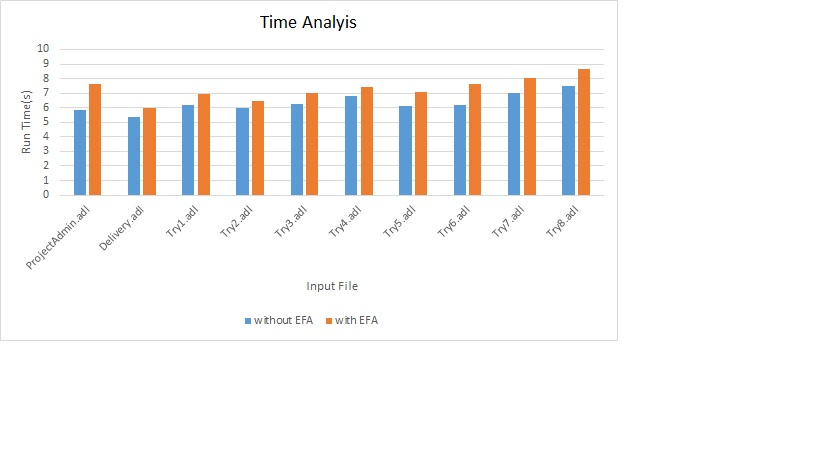
\includegraphics[width=1.3\textwidth]{./Chart1}
\caption{Run Time chart for test case 1 to 10.}~\label{fig:figure1}
\end{figure}


\begin{figure}
  \centering
    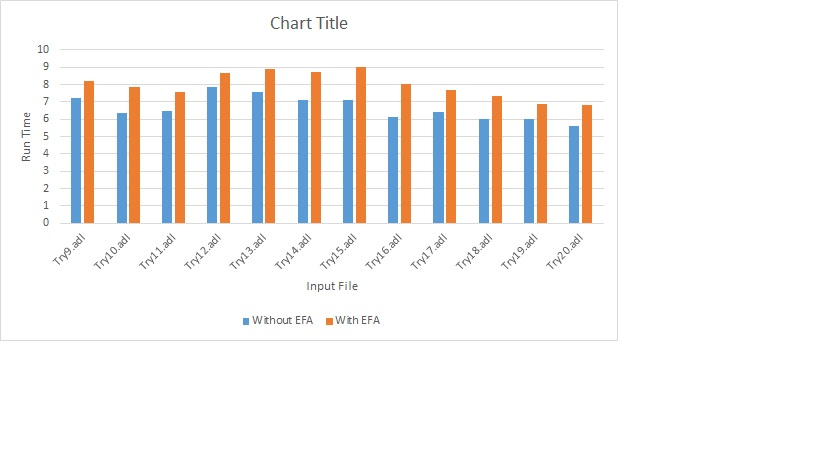
\includegraphics[width=1.3\textwidth]{./Chart2}
\caption{Run Time chart for test case 11 to 22.}~\label{fig:figure2}
\end{figure}

After measuring the performance of the current version of Ampersand compared to the EFA project we found out that there is a overhead cost of generating SQL statements from the ECA rules. The average overhead time of running EFA project is 1.16 sec. 

Calculate using the formula : 
\begin{equation}
	Overhead Time(s) =\frac{\left ( \sum  Run Time with EFA - Run Time without EFA\right )}{ No. of Test Cases}
\end{equation}

Figure\ref{fig:figure1} and Figure\ref{fig:figure2} shows a comparison of running time for all the test cases. The overhead cost of integrating EFA into Ampersand will add roughly about 1 second to the time it takes to generate a prototype. However the overall running time is still under 9 seconds for all the test cases so the waiting time for the end user is still very small compared to cost and time required to create an information system otherwise.


\subsection{Robustness}
The language dependency of using Haskell for this project allows the Developers to pattern match against all possible inputs. The Project was tested using the `' - -Wall'' flag to turn on all the warning options in Haskell. This allowed the team to pattern match against all possible inputs, this way the project does not rely on the test cases reachable through the Ampersand test input files.	


%
%\begin{longtable}{|L{1cm}|L{1.5cm}|L{1.5cm}|L{3.5cm}|L{4cm}|L{2cm}|L{1.5cm}|}
%\hline
%\textbf{No.} & \textbf{Test Case}  & \textbf{Initial State} & \textbf{Input} & \textbf{Expected Output} & \textbf{Actual Output} & \textbf{Result}\\
%\hline
%1.1 & User Registration & Landing page. Empty fields. & Email and passwoinrd entered. Clicks register. & Redirected to application main page. & As expected. & PASS \\
%\hline
%1.2 & User Registration & Landing page. Empty fields. & Empty field(s). Clicks register. & Stays on the same page. Error message appears. Empty field is highlighted. & As expected. & PASS \\
%\hline
%1.3 & User Registration & Landing page. Empty fields. & Email address already stored in database. Clicks register. & Stays on the same page. Error message appears. Email field is highlighted. & As expected. & PASS \\
%\hline
%\end{longtable}


%%\clearpage
\printglossaries
\bibliographystyle{alpha}
\bibliography{}

\end{document}

%%  LocalWords:  UML
